\documentclass[]{article}
\usepackage{xcolor,listings}
\usepackage{textcomp}
\usepackage[margin=1.0 in]{geometry}
\usepackage{graphicx}
\usepackage{biblatex}
\usepackage{hyperref}
\usepackage{subcaption}
\usepackage{amssymb}
\usepackage{lscape}
\usepackage{amsmath}
\usepackage{rotating}
\definecolor{light-gray}{gray}{0.95}
\newcommand{\code}[1]{\colorbox{light-gray}{\texttt{#1}}}
\title{DNN model evaluation metrics}
\author{Lacey Conrad\\DNN Research\\ Regis University}
\date{July, 2021}

\begin{document}
	\maketitle


\section{To Do}
\begin{itemize}
\item Continue reading mAP information
\item Continue researching specific metrics used in object detection
\item investigate visual means of displaying model metrics
\item Create example code snippets that can be used to calculate the more common metrics
\item Create code that can extract test tensor data in array form from model output.   Specifically need predicated and correct labels of test data.  
\end{itemize}
\section{Commonly used metrics}
\textbf{KEY}
\begin{itemize}
\item P positive instances of a condition 
\item N negative instances of a condition
\item TP true positive
\item TN true negative
\item FP false positive
\item FN false negative
\end{itemize}
\subsection{Confusion Matrix}
\textbf{NOTE:} 
\subsection{IoU}

 IoU metric determines how many objects were detected correctly and how many false positives were generated (will be discussed below).  It is quite literally defined as the intersection over union of the detection bounding box and the ground truth bounding box.  It is calculated by dividing the area of overlap between predicted bounding box and ground truth by the area of their union.\\

$IoU = \dfrac{\text{area of overlap}}{\text{area of union}}$
\\
or
\\

$IoU = \dfrac{true positive}{true positive + false positive + false negative}$\\

An Intersection over Union score $>$ 0.5 is normally considered a “good” prediction(Wadawadagi, 2020).

Intersection over Union is a ratio between the intersection and the union of the predicted boxes and the ground truth boxes. This stat is also known as the Jaccard Index and was first published by Paul Jaccard in the early 1900s.

Now for each class, the area overlapping the prediction box and ground truth box is the intersection area and the total area spanned is the union.

To get the intersection and union values, we first overlay the prediction boxes over the ground truth boxes. (see image)

\begin{figure}[!h]
	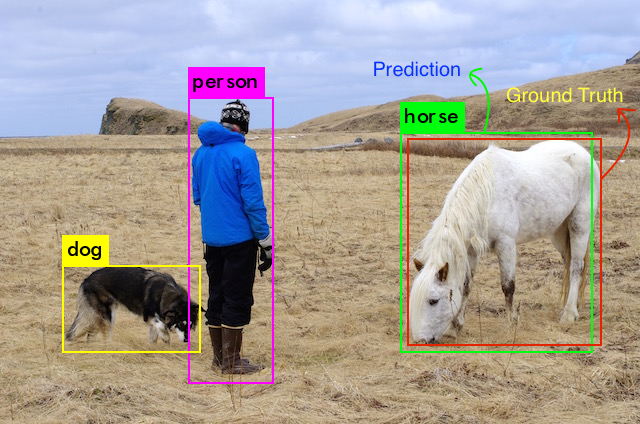
\includegraphics[scale=0.75]{iou2}
	\caption{A visual representation of the IoU.  For the horse, see how there is a box for the prediction, and another box for the ground truth (Shah, 2018).}
	\label{Fig:Race}
\end{figure}
\pagebreak
The intersection and union for the horse class in the above would look like this: 

\begin{figure}[!h]
	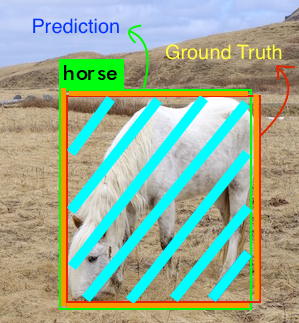
\includegraphics[scale=0.75]{iou3}
	\caption{The cross lines indicate the intersection (Shah, 2018).}
	\label{Fig:Race}
\end{figure}


\begin{figure}[!h]
	\includegraphics[scale=0.75]{iou}
	\caption{A visual representation of the IoU.  The green and blue boxes are machine predictions and the numbers are what the IoU values would be for that prediction (Wadawadagi, 2020).}
	\label{Fig:Race}
\end{figure}

\subsection{Precision}

Precision measures how accurate your predictions are. i.e. the percentage of your predictions that are correct.

$Precision = \dfrac{\text{true positive}}{\text{true positive + false positive}}$

\subsection{Recall}

Recall measures how good you find all the positives. 

$Recall = \dfrac{\text{true positive}}{\text{true positive + false negative}}$


\begin{figure}[!h]
	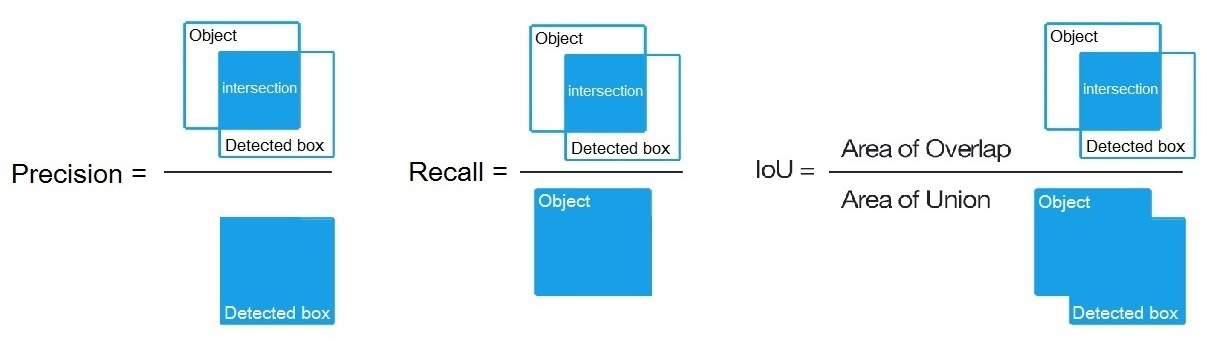
\includegraphics[scale=0.35]{pre_rec_iou}
	\caption{Difference between precision, recall, and IoU (Wadawadagi, 2020).}
	\label{Fig:Race}
\end{figure}

\subsection{F1 Score}

F1 score is HM (Harmonic Mean) of precision and recall.


$F_1 = 2 \times \dfrac  {\text{precision * recall}}{\text{precision + recall}}$
\subsection{Average precision (AP)}


\subsection{Mean average precision (mAP)}
\textbf{NOTE:} mAP is not calculated by taking the average of precision values!!!
\\
$mAP = \dfrac{\sum_{q=1}^Q \overline{P}(q)}{Q}$
\\
where:

Q = number of queries in the set\\
$\overline{P}(q)=average precision$
\\

What the formula is essentially telling us is that, for a given query, q, we calculate its corresponding AP, and then the mean of the all these AP scores would give us a single number, called the mAP, which quantifies how good our model is at performing the query.

In some contexts, AP is calculated for each class and averaged to get the mAP. But in others, they mean the same thing. For example, for COCO challenge evaluation, there is no difference between AP and mAP.

The mean Average Precision or mAP score is calculated by taking the mean AP over all classes and/or overall IoU thresholds, depending on different detection challenges that exist.

\begin{figure}[!h]
	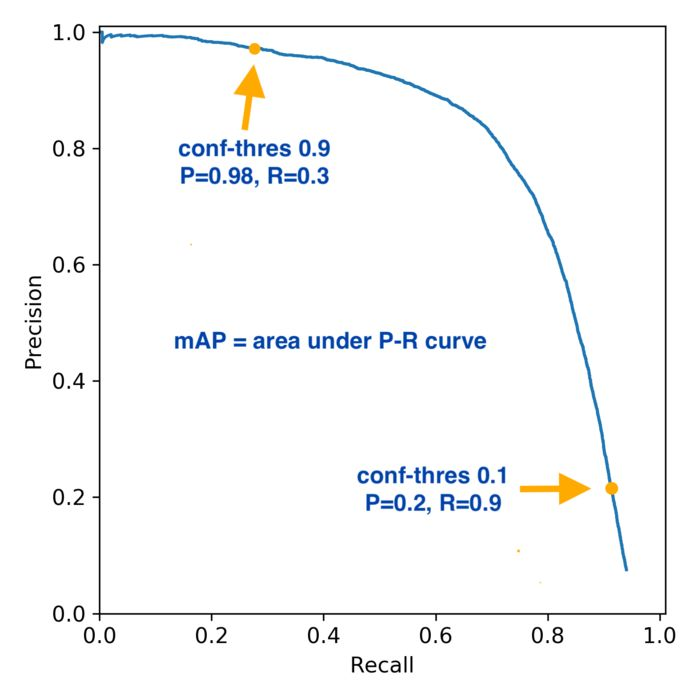
\includegraphics[scale=0.95]{map}
	\caption{mAP analysis (Wadawadagi, 2020).}
	\label{Fig:Race}
\end{figure}



\section{How to decide which metrics to use}
For the best possible analysis, use both a validation set (data set that is used to tune hyper-parameters) and test set (data set that is used to assess the performance of a fully-trained model) (Wadawadagi, 2020).
\begin{itemize}
\item Validation metrics
\begin{itemize}
\item Use mAP to select the best performing model (model that is more stable and consistent) out of all the trained weights across iterations/epochs. Use mAP to understand whether the model should be trained/tuned further or not.
\item Check class level AP values to ensure the model is stable and good across the classes.
\item As per use-case/application, if you're completely tolerant to FNs and highly intolerant to FPs then to train/tune the model accordingly use Precision.
\item As per use-case/application, if you're completely tolerant to FPs and highly intolerant to FNs then to train/tune the model accordingly use Recall (Wadawadagi, 2020).
\end{itemize}
\item Testing metrics
\begin{itemize}
\item If you're neutral towards FPs and FNs, then use F1 score to evaluate the best performing model.
\item If FPs are not acceptable to you (without caring much about FNs) then pick the model with higher Precision
\item If FNs are not acceptable to you (without caring much about FPs) then pick the model with higher Recall
\item Once you decide metric you should be using, try out multiple confidence thresholds (say for example - 0.25, 0.35 and 0.5) for given model to understand for which confidence threshold value the metric you selected works in your favour and also to understand acceptable trade off ranges (say you want Precision of at least 80\% and some decent Recall). Once confidence threshold is decided, you use it across different models to find out the best performing model (Wadawadagi, 2020).
\end{itemize}
\end{itemize}

\begin{table}[!h]
	\begin{center}
		\caption{Metrics to use on testing and validation data according to FP/FN importance.}
		\label{tab:table1}
		\begin{tabular}{|c|c|c|}
			\hline
			False Positive & False Negative & Metric to focus on\\
			\hline
		$\sim$ &$\sim$ & F1\\
			$\Downarrow$ &$\sim$ & Maxmimize precision\\
		$\sim$ &$\Downarrow$ & Maximize recall\\
			\hline
			
			\hline
		\end{tabular}
	\end{center}
\end{table}

\section{Helpful research papers and other references}
\begin{itemize}
\item visualizing feature maps 
(may be able to help show how to dissect data at each layer and for each model child)

\url{https://ravivaishnav20.medium.com/visualizing-feature-maps-using-pytorch-12a48cd1e573}

\item mAP (mean average precision) might confuse you!
Shows examples of a lot of the other important computer vision metrics commonly used.

\url{https://towardsdatascience.com/map-mean-average-precision-might-confuse-you-5956f1bfa9e2}

\item mAP (mean Average Precision) for Object Detection
Very concise description of mAP.

\url{https://jonathan-hui.medium.com/map-mean-average-precision-for-object-detection-45c121a31173}

\item Breaking down mean average precision (mAP)
Explains how IoU and mAP are related and gives good examples

\url{https://towardsdatascience.com/breaking-down-mean-average-precision-map-ae462f623a52}
\end{itemize}
\section{References}
\begin{enumerate}
	
	\item Shah, T. (2018, October 17). Measuring object detection models — mAP — What is mean average precision? Medium. 
	
	\url{https://towardsdatascience.com/what-is-map-understanding-the-statistic-of-choice-for-comparing-object-detection-models-1ea4f67a9dbd}
	
\item	Tan, R. J. (2020, July 6). Breaking down mean average precision (map). Medium.

 \url{https://towardsdatascience.com/breaking-down-mean-average-precision-map-ae462f623a52}
	
	\item Wadawadagi, V. (2020). Metrics to use to evaluate deep learning object detectors. KDnuggets. \url{https://www.kdnuggets.com/2020/08/metrics-evaluate-deep-learning-object-detectors.html}
	

\item Yohanandan, S. (2020, June 9). Map (mean average precision) might confuse you! Medium. \url{https://towardsdatascience.com/map-mean-average-precision-might-confuse-you-5956f1bfa9e2}

\end{enumerate}
\end{document}